\documentclass[UTF8]{beamer}
\usetheme{Madrid}
\usefonttheme[onlymath]{serif}
%\usecolortheme{}

\usepackage{ctex}
\usepackage{graphicx}
\usepackage{subfigure}
\usepackage{braket}

%information
\title{Husimi图}
\author{邴泓霖}

\begin{document}
\frame{\titlepage}
\begin{frame}\frametitle{目录}
    \tableofcontents
\end{frame}
%----------------------------------------------------------%
%
\section{论文中基本概念的梳理}
\subsection{流算符}
\begin{frame}\frametitle{流算符}
    在量子力学的课本中,在某一点的概率流算符(the probability flux)算符可以定义为
    \begin{equation}
        \hat{\mathbf{j}}_{\mathbf{r}} = \frac{1}{2m}(\ket{\mathbf{r}}\bra{\mathbf{r}}\hat{\mathbf{p}}+\hat{\mathbf{p}}\ket{\mathbf{r}}\bra{\mathbf{r}})           
        \label{flux:def}
    \end{equation}
    其中$\mathbf{r}$和$\mathbf{p}$分别是质量为$m$的粒子的位置和动量。
    
    同时,可以计算出概率流算符的平均值
    \begin{equation}
        \begin{aligned}
            \bra{\psi}\hat{\mathbf{j}}_{\mathbf{r}}\ket{\psi}&=
            \frac{\mathrm{i}\hbar}{2m}(
            \mathrm{\psi}(\mathbf{r})\nabla\mathrm{\psi}^{*}(\mathbf{r})
            -\mathrm{\psi}^{*}(\mathbf{r})\nabla\mathrm{\psi}(\mathbf{r})
            )\\
            &=\frac{1}{m}\Im[\mathrm{\psi}^{*}(\mathbf{r})(-\mathrm{i}\hbar\nabla)\mathrm{\psi}(\mathbf{r})]\\ 
            &=\frac{1}{m}\Im[\mathrm{\psi}^{*}(\mathbf{r})\hat{\mathbf{p}}\mathrm{\psi}(\mathbf{r})]
            \label{flux:ave}
        \end{aligned}
    \end{equation}
\end{frame}
\begin{frame}\frametitle{流算符的“矛盾”}
    从式(\ref{flux:ave})可以看出流算符的概念有一些“矛盾”,我们知道位置很精确的同时,还需要一些关于动量的信息。\\
    \begin{block}{原文}
        The concept of “flux at a point” seems paradoxical because we say something about momentum while also knowing position precisely.
    \end{block}
\end{frame}
\begin{frame}\frametitle{造成“矛盾”的原因}
    \begin{block}{Heisenberg不确定性原理}
        \Large
        \begin{center}
            $\Delta x \, \Delta p \geqslant \frac{\hbar}{2}$
        \end{center}
    \end{block}
\end{frame}
%
\begin{frame}\frametitle{流算符}
    对于传统的流算符,存在如下问题:
    \begin{itemize}
        \item 概率流是否可以被测量
        \item 具有时间反演对称性的系统,其概率流会消失。
    \end{itemize}
\end{frame}
%-------------------------------------------------------------%
\subsection{流算符的本征态}
\begin{frame}
    高斯型基矢可以写为
    \begin{equation}
        \braket{\mathbf{r}|\mathbf{r}_0,\sigma}=N_{_\sigma}^{d/2}\mathrm{e}^{-\frac{(\mathbf{r}-\mathbf{r}_{_0})^2}{4\sigma^2}}
    \end{equation}
    将式(\ref{flux:def})改写成
    \begin{equation}
        \hat{\mathbf{j}}_{\mathbf{r}_0,\sigma} = \frac{1}{2m}(\ket{\mathbf{r}_0,\sigma}\bra{\mathbf{r}_0,\sigma}\hat{\mathbf{p}}+\hat{\mathbf{p}}\ket{\mathbf{r}_0,\sigma}\bra{\mathbf{r}_0,\sigma})           
        \label{flux:sigma}
    \end{equation}
\end{frame}
\begin{frame}\frametitle{流算符的本征态}
    写出本征方程:
    \begin{equation}
        \hat{\mathbf{j}}_{\mathbf{r}_0,\sigma,i}\,\ket{\lambda_{\sigma,i}}=\lambda_{\sigma,i}\ket{\lambda_{\sigma,i}} 
        \label{flux:eigeq}
    \end{equation}
    式(\ref{flux:sigma})与(\ref{flux:eigeq})中的$i$是空间的维度指标。
    该本征方程的解可以写为
    \begin{equation*}
        \ket{\lambda_{\sigma,i}}=\ket{\mathbf{r}_0,\sigma}+a\hat{p}_i\ket{\mathbf{r}_0,\sigma}
    \end{equation*}
    可以将求解本征方程转换成:
    \begin{equation}
        \hat{\mathbf{j}}_{\mathbf{r}_0,\sigma}\ket{\lambda_{\sigma,i}} =
        \frac{1}{2m}(a\braket{\hat{p}_i^2}_{\sigma}\ket{\mathbf{r}_0,\sigma}+\hat{p}_i\ket{\mathbf{r}_0,\sigma})
    \end{equation}
\end{frame}
\begin{frame}\frametitle{流算符的本征态}
    由于$\braket{\hat{p}_i^2}_{\sigma}=\frac{\hbar^2}{4\sigma^2}$因此有两个本征值可写为
    \begin{equation}
        \lambda_{\sigma,i,\pm}=\pm\frac{\hbar}{4m\sigma}
    \end{equation}
    本征态在坐标表象的形式如下
    \begin{equation}
        \braket{\mathbf{r}|\lambda_{\sigma,i,\pm}}=
        \braket{\mathbf{r}|\mathbf{r}_0,\sigma}\pm
        \frac{\mathrm{i}}{\sigma}\mathbf{e}_i\cdot(\mathbf{r}-\mathbf{r}_0)\braket{\mathbf{r}|\mathbf{r}_0,\sigma}
        \label{husimi:eigstate}   
    \end{equation}
\end{frame}
\begin{frame}
    \frametitle{谐振子的本征态}
    \begin{align}
        \braket{\mathbf{r}|0}&=\braket{\mathbf{r}|\mathbf{r}_0,\sigma}\\
        \braket{\mathbf{r}|1}&=\frac{\mathrm{e}_i\cdot(\mathbf{r}-\mathbf{r}_0)}{\sigma}\braket{\mathbf{r}|\mathbf{r}_0,\sigma}\\
        \vdots 
    \end{align}
\end{frame}
\begin{frame}
    \frametitle{流算符和本征态的矩阵表示}
    流算符:
    \begin{equation*}
        \hat{j}_{\mathbf{r}_0,\sigma,i}=
        \begin{bmatrix}
            0                 &+\mathrm{i}\lambda&0\cdots&0\\
            -\mathrm{i}\lambda&0                 &0\cdots&0\\
            0                 &0                 &0\cdots&0\\
            \vdots            &\vdots            &\ddots &\vdots \\
            0                   &0               &\cdots&0    
        \end{bmatrix}
    \end{equation*}
    本征态:
    \begin{equation*}
        \ket{\lambda_{1}}=
        \begin{bmatrix}
            1\\
            -\mathrm{i}\\
            0\\
            \vdots
        \end{bmatrix}
        \ket{\lambda_{2}}
        \begin{bmatrix}
            1\\
            \mathrm{i}\\
            0\\
            \vdots
        \end{bmatrix}
        \ket{\lambda_{3}}
        \begin{bmatrix}
            0\\
            0\\
            0\\
            \vdots
        \end{bmatrix}
        \cdots
    \end{equation*}
\end{frame}
\begin{frame}
    \frametitle{拓展后的流算符}
    
    

\end{frame}
%-----------------------------------------------------------%
\subsection{流算符的测量}
\begin{frame}\frametitle{流算符的测量}

\end{frame}
%------------------------------------------------------------%
%
\section{Husimi表象}
\begin{frame}\frametitle{Husimi表象}
    
\end{frame}
%-------------------------------------------------------------%
%
%-------------------------------------------------------------%
\section{复现的结果}
\subsection{未处理的Husimi图}
\begin{frame}
    \frametitle{$\psi_A$的模仿}
    \begin{figure}[h]
        \centering
        \subfigure[$ 2\% $]{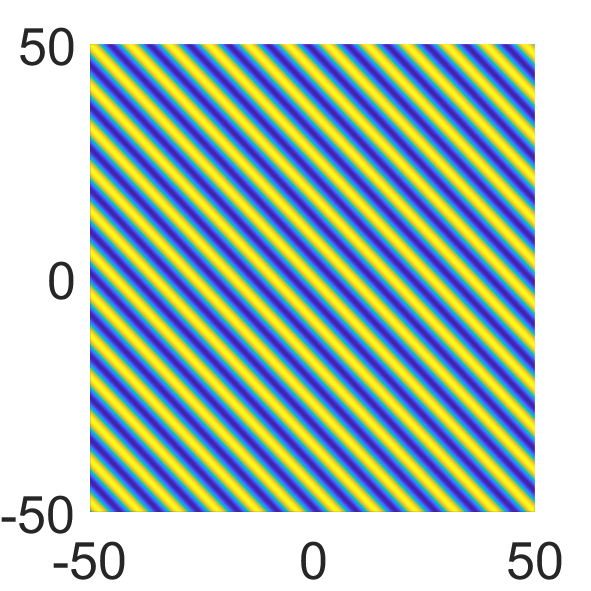
\includegraphics[width = 0.22\textwidth]{../figure/PsiA2.png}}
        \subfigure[$ 10\%$]{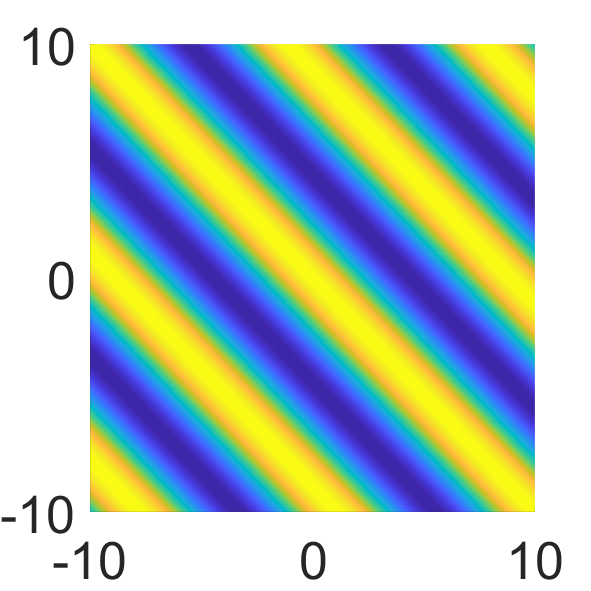
\includegraphics[width = 0.22\textwidth]{../figure/PsiA10.png}}
        \subfigure[$ 50\% $]{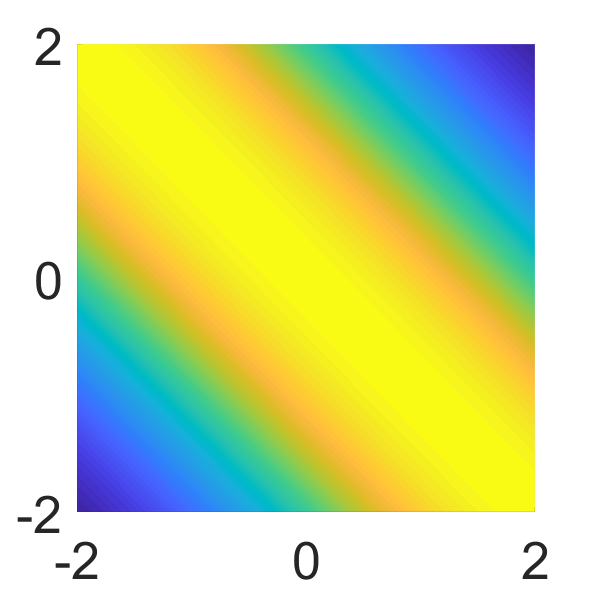
\includegraphics[width = 0.22\textwidth]{../figure/PsiA50.png}}
        \subfigure[$ 250\% $]{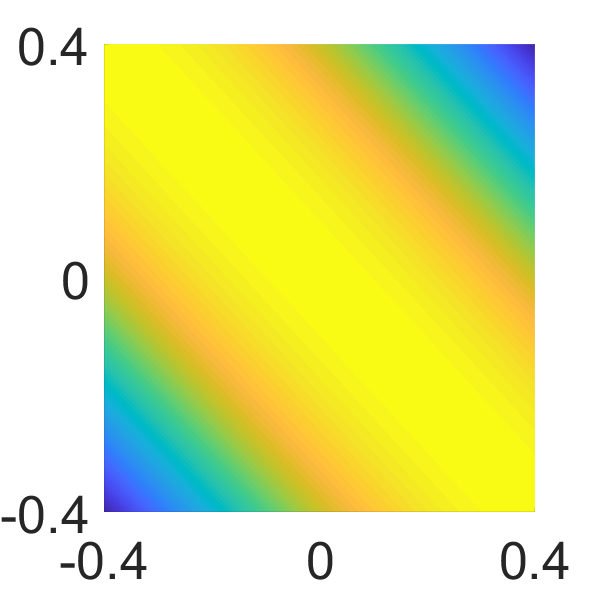
\includegraphics[width = 0.22\textwidth]{../figure/PsiA250.png}}
        \caption{$|\psi_A|^2$} 
    \end{figure}
\end{frame}
\begin{frame}\frametitle{$\psi_B$的Husimi图}
    \begin{figure}[h]
        \centering
        \subfigure[$ 2\%$]{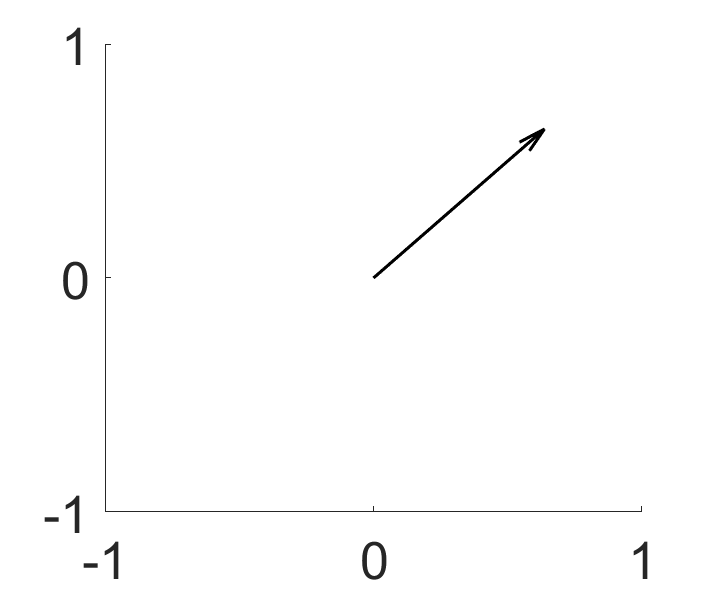
\includegraphics[width = 0.22\textwidth]{../figure/HuA2.png}}
        \subfigure[$ 10\% $]{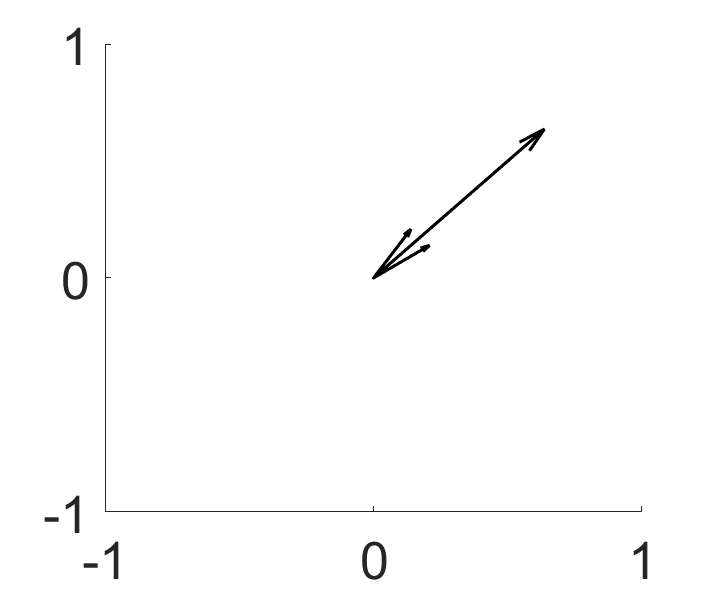
\includegraphics[width = 0.22\textwidth]{../figure/HuA10.png}}
        \subfigure[$ 50\% $]{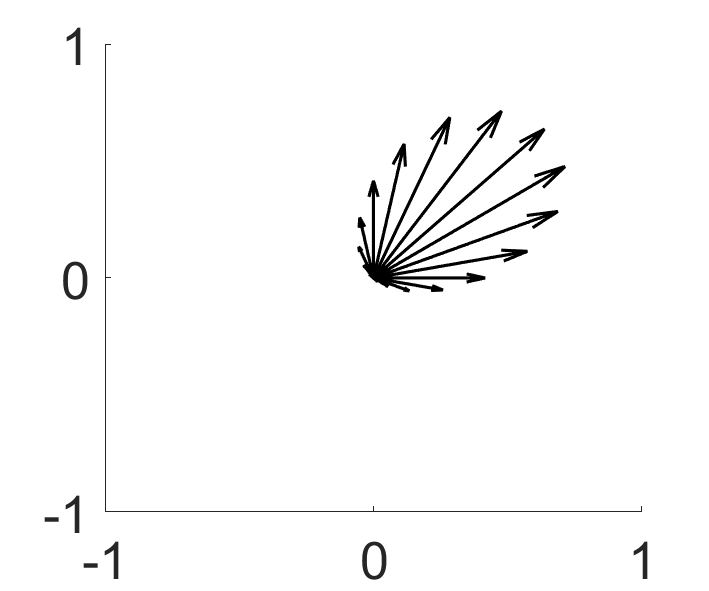
\includegraphics[width = 0.22\textwidth]{../figure/HuA50.png}}
        \subfigure[$ 250\% $]{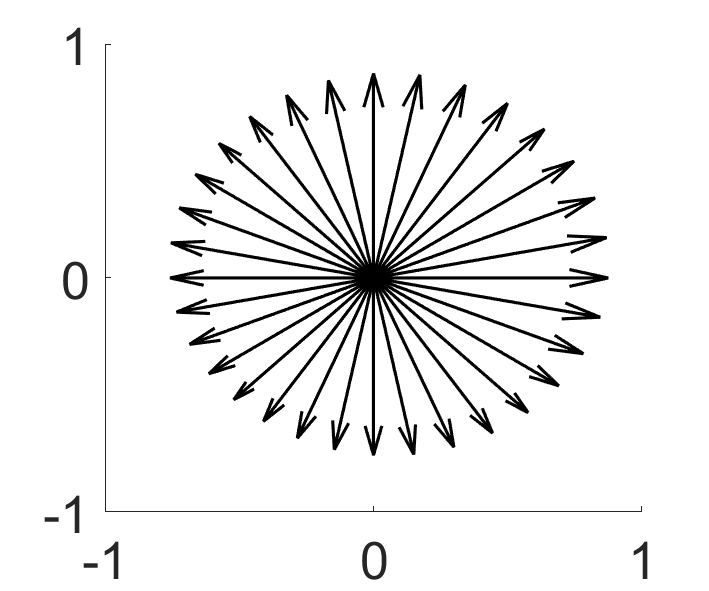
\includegraphics[width = 0.22\textwidth]{../figure/HuA250.png}}
        \caption{Husimi图}
    \end{figure}
\end{frame}
\begin{frame}
    \frametitle{$\psi_B$的模仿}
    \begin{figure}[h]
        \centering
        \subfigure[$ 2\% $]{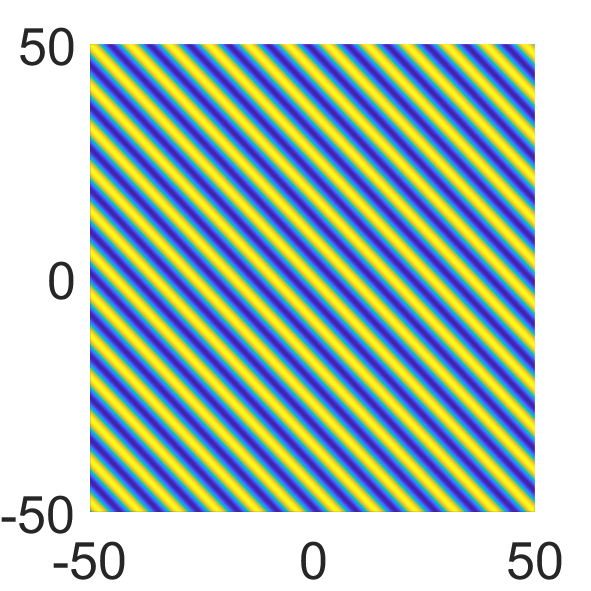
\includegraphics[width = 0.22\textwidth]{../figure/PsiB2.png}}
        \subfigure[$ 10\%$]{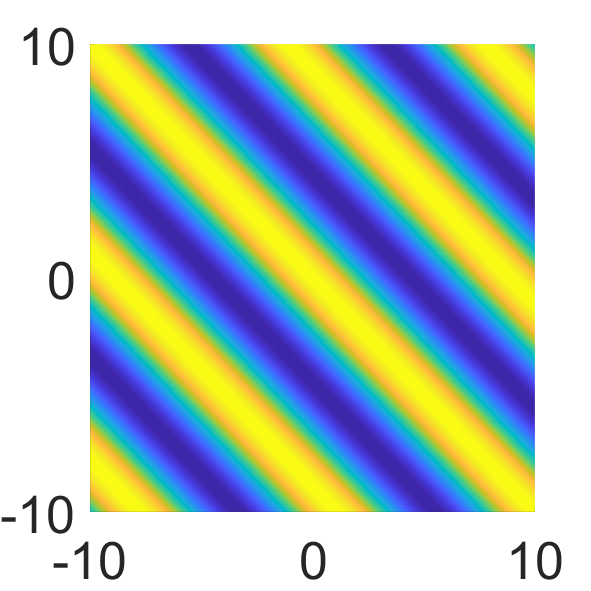
\includegraphics[width = 0.22\textwidth]{../figure/PsiB10.png}}
        \subfigure[$ 50\% $]{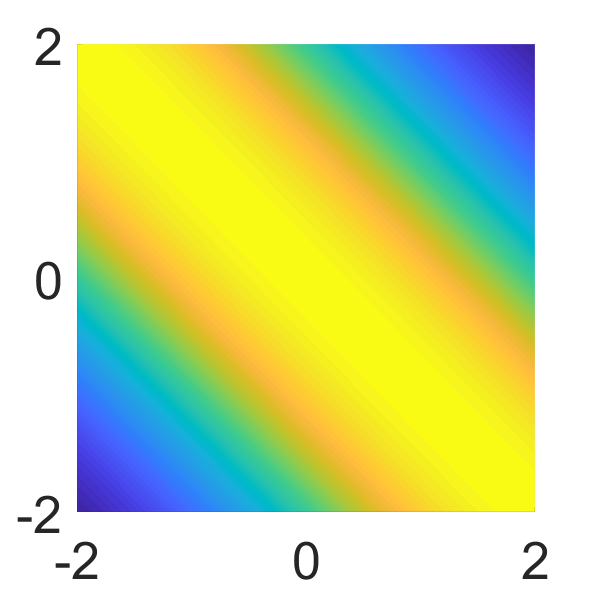
\includegraphics[width = 0.22\textwidth]{../figure/PsiB50.png}}
        \subfigure[$ 250\% $]{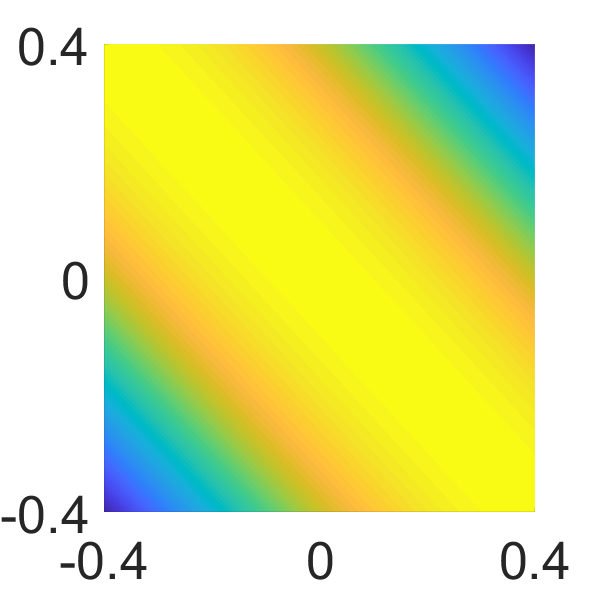
\includegraphics[width = 0.22\textwidth]{../figure/PsiB250.png}}
        \caption{$ |\psi_B|^2$} 
    \end{figure}
\end{frame}
\begin{frame}\frametitle{$\psi_B$的Husimi图}
    \begin{figure}[h]
        \centering
        \subfigure[$ 2\%$]{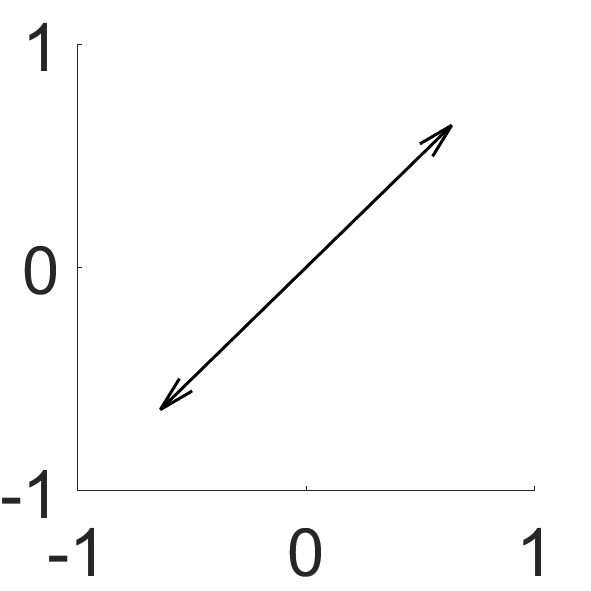
\includegraphics[width = 0.22\textwidth]{../figure/HuB2.png}}
        \subfigure[$ 10\% $]{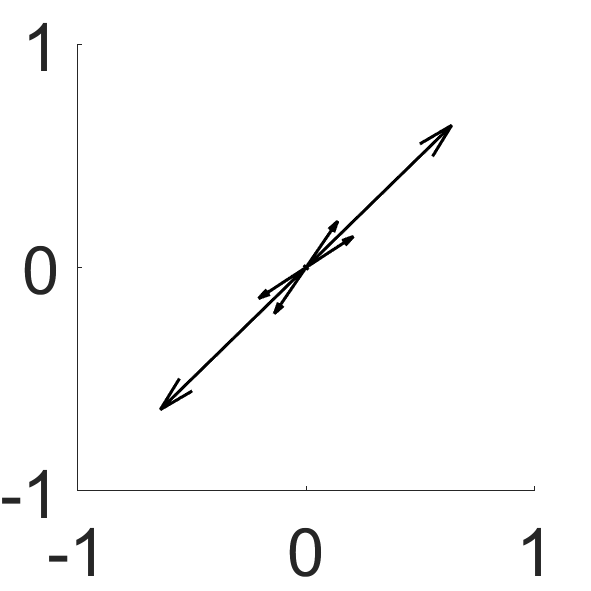
\includegraphics[width = 0.22\textwidth]{../figure/HuB10.png}}
        \subfigure[$ 50\% $]{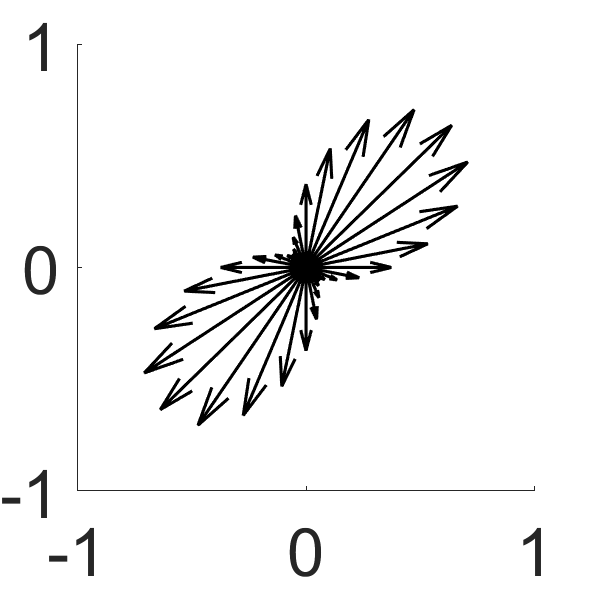
\includegraphics[width = 0.22\textwidth]{../figure/HuB50.png}}
        \subfigure[$ 250\% $]{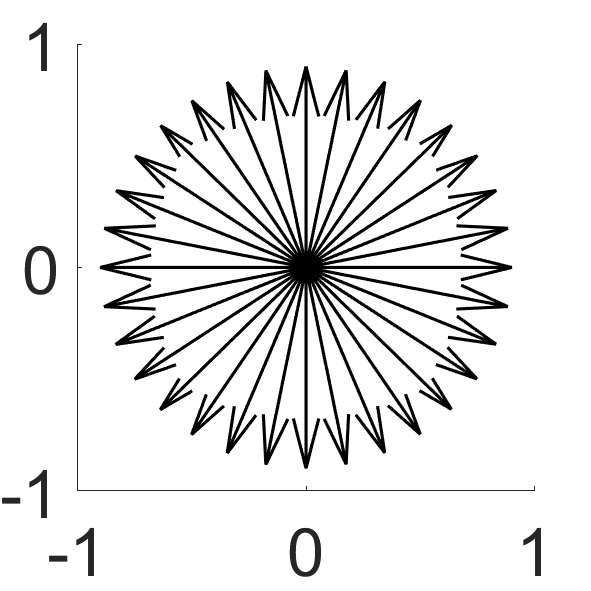
\includegraphics[width = 0.22\textwidth]{../figure/HuB250.png}}
        \caption{Husimi图}
    \end{figure}
\end{frame}
\begin{frame}\frametitle{$\Psi_C$的重複結果}
    \begin{figure}[h]
        \centering
        \subfigure[$ \Delta k /k = 30\%$ 時的Husimi圖]{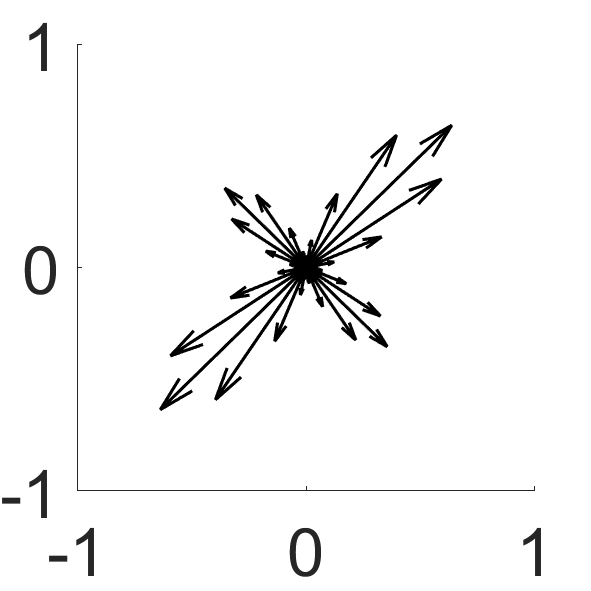
\includegraphics[width = 0.4\textwidth]{../figure/HuC30.png}}
        \subfigure[$ \Psi_C $的模方]{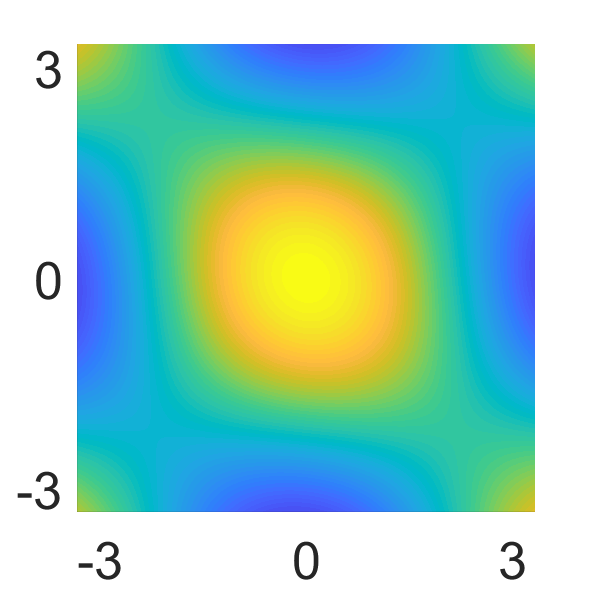
\includegraphics[width = 0.4\textwidth]{../figure/PsiC30.png}}
        \caption{Husimi图}
    \end{figure}
\end{frame}
%
%--------------------------------------------------------------%
\subsection{处理过的Husimi图}
\begin{frame}

\end{frame}
\end{document}